\subsection*{Ejercicio 5. Programación y Filtrado}

Una señal no estacionaria es aquella cuyas propiedades estadísticas (frecuencia, amplitud) varían con el tiempo. Para estas señales, una sola FFT ``promedia'' todo el tiempo y pierde la información de cuándo ocurrieron los eventos.

Programe en Python las siguientes funciones en un dominio de 2 segundos ($f_s = 1000$ Hz):
\begin{enumerate}
    \item \textbf{Señal A (Chirp):} $s_1(t) = \sin(2\pi(10 + 40t)t)$. (Frecuencia que sube de 10 a 90 Hz).
    \item \textbf{Señal B (Salto de Frecuencia):} $s_2(t) = \sin(2\pi 20t)$ para $t < 1\text{s}$, y $s_2(t) = \sin(2\pi 80t)$ para $t \geq 1\text{s}$.
\end{enumerate}

\textbf{Requerimientos del Código:}
\begin{itemize}
    \item Calcule y grafique la FFT de ambas señales. Observe cómo en la Señal B aparecen dos picos, pero se pierde la noción de qué frecuencia va primero.
    \item Aplique un filtro pasa-altas con corte en 50 Hz a ambas señales en el dominio de la frecuencia.
    \item Realice la IFFT y grafique el resultado en el tiempo. Describa qué sucede con la parte inicial de la Señal B tras el filtrado.
\end{itemize}

\vspace{0.5cm}

\textbf{Solución:}


En primera instancia se calculan y grafican las transformadas de Fourier de ambas señales para poder observar el espectro de frecuencias y como este se distribuye en el dominio de la frecuencia. Si observamos la Señal B, se aprecian con total claridad dos picos dominantes en las frecuencias de $20\text{ Hz}$ y $80\text{ Hz}$, sin embargo, como la transformada de Fourier integra la señal a lo largo de todo el intervalo y la magnitud del espectro termina actuando como un promedio de todas las oscilaciones. Entonces aunque el espectro nos dice que frecuencias están presentes pierde la información de cuando aparecieron donde si miramos la gráfica de magnitud, es imposible saber si el pulso de $20\text{ Hz}$ ocurrió antes que el de $80\text{ Hz}$, si fue al revés, o si ambos tonos sonaron al mismo tiempo durante toda la simulación.

Por otra parte, el filtrado de la señal en el dominio de la frecuencia ofrece resultados muy predecibles y consistentes con la teoría esto es por que aplica un filtro pasa-altas ideal con una frecuencia de corte estricta en $50\text{ Hz}$ así se elimina cualquier componente espectral por debajo de ese límite y como el primer segundo de la Señal B consistía únicamente en un tono puro de $20\text{ Hz}$, esta primera mitad de la señal es eliminada por completo por el filtro.

Como consecuencia al aplicar la Transformada Inversa para regresar la señal manipulada al dominio del tiempo notamos cómo la primera mitad del vector prácticamente desaparece. La amplitud entre $t=0$ y $t=1\text{ s}$ es casi cero, mostrando un decaimiento, mientras que a partir de $t=1\text{ s}$ la señal de $80\text{ Hz}$ se mantiene intacta tras haber superado el corte del filtro. 

Cabe mencionar que justo en la discontinuidad de $t=1\text{ s}$ aparecen unas pequeñas oscilaciones que se deben al fenómeno de Gibbs que surge al multiplicar el espectro por una función escalón rectangular, la cual requeriría un ancho de banda infinito para recrear un cambio tan abrupto en el tiempo de forma perfecta.

\begin{minted}[bgcolor=lightgray!20, fontsize=\small, linenos]{python}
import numpy as np
import matplotlib.pyplot as plt
from numpy.fft import fft, ifft, fftfreq

# Parámetros
fs = 1000
T = 2.0
t = np.linspace(0, T, int(fs * T), endpoint=False)
N = len(t)

# Señal A (Chirp): s1(t) = sin(2*pi*(10 + 40t)*t)
s1 = np.sin(2 * np.pi * (10 + 40 * t) * t)

# Señal B (Salto de Frecuencia): 
# s2(t) = sin(2*pi*20*t) para t < 1, y sin(2*pi*80*t) para t >= 1
s2 = np.piecewise(t, [t < 1, t >= 1], [
    lambda t: np.sin(2 * np.pi * 20 * t), 
    lambda t: np.sin(2 * np.pi * 80 * t)
])

# Transformada de Fourier
S1 = fft(s1)
S2 = fft(s2)
freqs = fftfreq(N, 1/fs)

# Filtro Pasa-Altas
cutoff = 50
high_pass_filter = np.abs(freqs) >= cutoff

# Aplica el filtro en el dominio de la frecuencia
S1_filtered = S1 * high_pass_filter
S2_filtered = S2 * high_pass_filter

# Aplica la Transformada Inversa para obtener señales filtradas en el tiempo
s1_filtered = np.real(ifft(S1_filtered))
s2_filtered = np.real(ifft(S2_filtered))
\end{minted}

\begin{figure}[H]
    \centering
    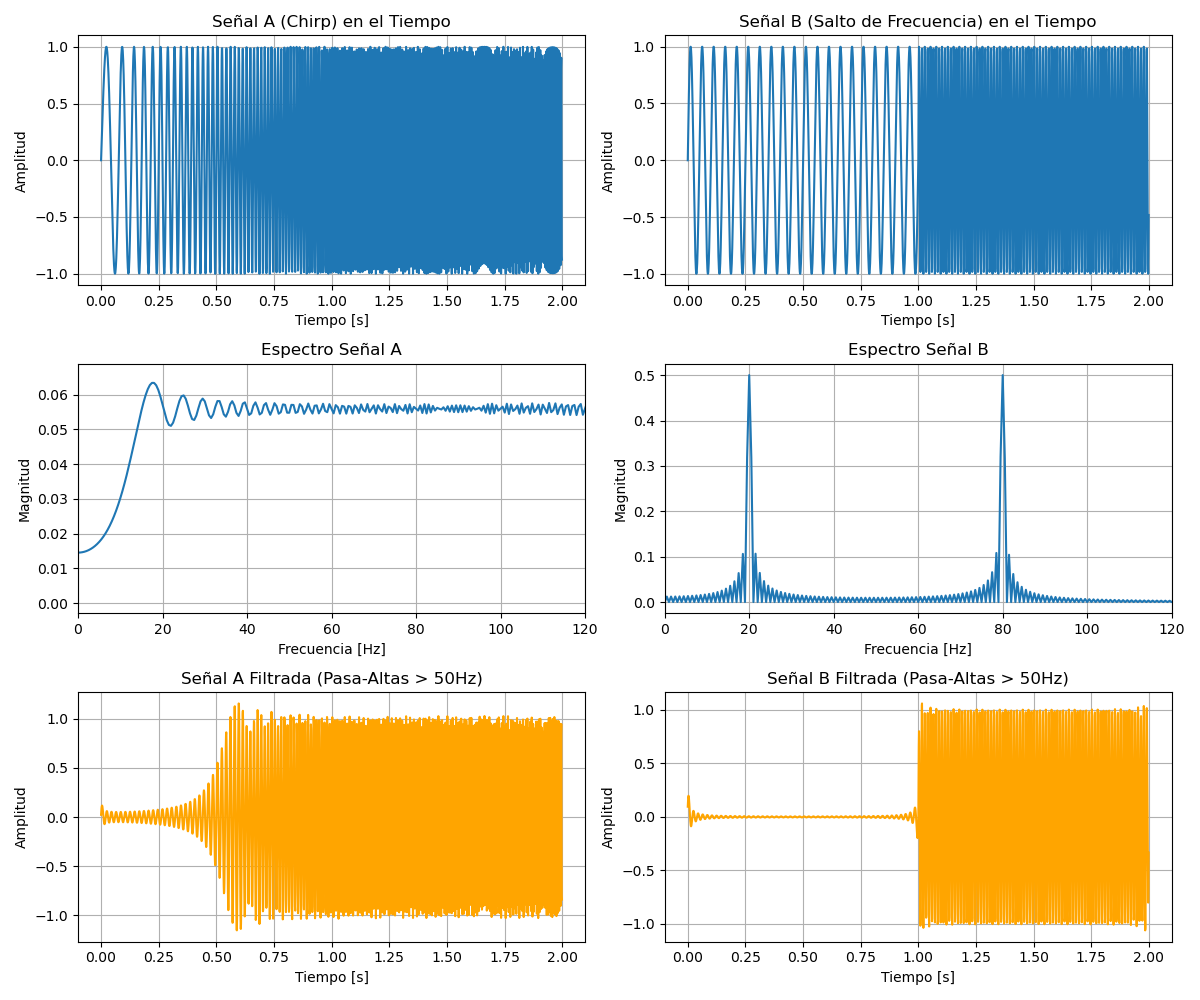
\includegraphics[width=\textwidth]{ejercicio5_grafica.png}
    \caption{Señales en el tiempo, sus respectivos espectros de frecuencia y el resultado tras aplicar un filtro pasa-altas con corte en 50 Hz.}
    \label{fig:ejercicio5}
\end{figure}
